\chapter{Linux基础知识}


\section{操作系统和linux}
操作系统(Operating System,简称OS)传统上是负责对计算机硬件直接控制及管理的系统软件。操作系统的功能一般包括处理器管理、存储管理、文件管理、设备管理和作业管理等。当多个程序同时运行时,操作系统负责规划以优化每个程序的处理时间。

一个操作系统可以在概念上分割成两部分:内核(Kernel)以及壳(shell)。一个壳程序包裹了与硬件直接交流的内核:硬件<->内核<->壳<->应用程序。但有些操作系统上内核与壳完全分开(例如Unix、Linux等),这样用户就可以在一个内核上使用不同的壳;而另一些的内核与壳关系紧密(例如Microsoft Windows),内核及壳只是操作层次上不同而已。

Linux的出现,最早开始于一位名叫Linus Torvalds的计算机爱好者,当时他是芬兰赫尔辛基大学的学生。他的目的是想设计一个代替Minix(是由一位名叫Andrew Tannebaum的计算机教授编写的一个操作系统示教程序)的操作系统,这个操作系统可用于386、486或奔腾处理器的个人计算机上,并且具有Unix操作系统的全部功能,因而开始了Linux雏形的设计。 

Linux以它的高效性和灵活性著称。它能够在PC计算机上实现全部的Unix特性,具有多任务、多用户的能力。Linux是在GNU公共许可权限下免费获得的,是一个符合POSIX标准的操作系统。Linux操作系统软件包不仅包括完整的Linux操作系统,而且还包括了文本编辑器、高级语言编译器等应用软件。它还包括带有多个窗口管理器的X-Windows图形用户界面,如同我们使用Windows NT一样,允许我们使用窗口、图标和菜单对系统进行操作。 

Linux之所以受到广大计算机爱好者的喜爱,主要原因有两个,一是它属于自由软件,用户不用支付任何费用就可以获得它和它的源代码,并且可以根据自己的需要对它进行必要的修改,无偿对它使用,无约束地继续传播。另一个原因是,它具有Unix的全部功能,任何使用Unix操作系统或想要学习Unix操作系统的人都可以从Linux中获益。

通常情况下,Linux被打包成供个人计算机和服务器使用的Linux发行版,一些流行的主流Linux发布版,包括Debian(及其派生版本Ubuntu、Linux Mint)、Fedora(及其相关版本Red Hat Enterprise Linux、CentOS)和openSUSE等。Linux发行版包含Linux内核和支撑内核的实用程序和库,通常还带有大量可以满足各类需求的应用程序。个人计算机使用的Linux发行版通常包含XWindow和一个相应的桌面环境,如GNOME或KDE。桌面Linux操作系统常用的应用程序,包括Firefox网页浏览器、LibreOffice办公软件、GIMP图像处理工具等。由于Linux是自由软件,任何人都可以创建一个符合自己需求的Linux发行版。
\section{什么是Ubuntu}

Ubuntu是基于Debian发行版和GNOME桌面环境,与Debian的不同在于它每6个月会发布一个新版本(即每年的四月与十月),每2年发布一个LTS长期支持版本。普通的桌面版可以获得发布后18个月内的支持,标为LTS(长期支持)的桌面版可以获得更长时间的支持。为了稳定,我们一般采用LTS版本。

Ubuntu在安装完成以后,用户无需再费神安装浏览器、Office套装程序、多媒体播放程序等常用软件,一般也无需下载安装网卡、声卡等硬件设备的驱动(但部分显卡需要额外下载的驱动程序,且不一定能用包库中所提供的版本);
Ubuntu所有系统相关的任务均需使用Sudo指令是它的一大特色,这种方式比传统的以系统管理员账号进行管理工作的方式更为安全,此为Linux、Unix系统的基本思维之一。

Ubuntu的开发者与Debian和GNOME开源社区合作密切,其各个正式版本的桌面环境均采用GNOME的最新版本,通常会紧随GNOME项目的进展而及时更新。Ubuntu与Debian使用相同的deb软件包格式,可以安装绝大多数为Debian编译的软件包,虽然不能保证完全兼容,但大多数情况是通用的。

\section{操作系统的启动和安装}
操作系统越来越多,技术也日新月异,在探索安装多系统的过程中我们遇到许多问题,大概总结在这里。

\subsection{操作系统启动的相关知识}
安装双系统最大的问题一般都出在启动项上,如果对电脑正常的启动机制不够了解,非常容易误操作导致问题。所以有必要先了解一下相关知识。
(Win7及以前的系统参考BIOS+MBR,win8以后直接跳转到UEFI+GPT。如果你有兴趣不妨都看看。)
\subsubsection{BIOS+MBR}
对于BIOS+MBR,整个开机流程到操作系统之前的动作应该是这样的\footnote{引自《鸟哥Linux私房菜(第三版)》}:
\begin{enumerate}
	\item BIOS:开机主动执行的韧体\footnote{韧体就是写入到硬件上的一个软件程序},会认识第一个可开机的装置;
	\item MBR:第一个可开机装置的第一个扇区内的主要启动记录区块,内存开机管理程序;
	\item 开机管理程序(boot loader):一支可读取核心档案来执行的软件;
	\item 核心档案:开始操作系统的功能...
\end{enumerate}

由上面的说明我们会知道,BIOS与MBR都是硬件本身会支持的功能,至于Boot loader则是操作系统安装在MBR上面的一套软件了。由于MBR仅有446 bytes而已,因此这个开机管理程序是非常小而美的。这个boot loader的主要任务有底下这些项目:
\begin{itemize}
	\item 提供选单:用户可以选择不同的开机项目,这也是多重引导的重要功能!
	\item 载入核心档案:直接转向可开机的程序区段来开始操作系统;
	\item 转交其他loader:将开机管理功能转交给其他loader负责。
\end{itemize}

上面前两点还容易理解,但是第三点很有趣喔!那表示你的计算机系统里面可能具有两个以上的开机管理程序呢! 有可能吗?我们的硬盘不是只有一个MBR而已?是没错啦!但是开机管理程序除了可以安装在MBR之外, 还可以安装在每个分区的启动扇区(boot sector)喔!分区还有各别的启动扇区喔?没错啊!这个特色才能造就『多重引导』的功能啊!

我们举一个例子来说,假设你的个人计算机另有一个硬盘,里面切成四个分区,其中第一、二分区分别安装了Windows及Linux, 你要如何在开机的时候选择用Windows还是Linux开机呢?假设MBR内安装的是可同时认识Windows/Linux操作系统的开机管理程序,那举整个流程可以图标如下:

\begin{figure}[H]
	%\usepackage{float}
	\centering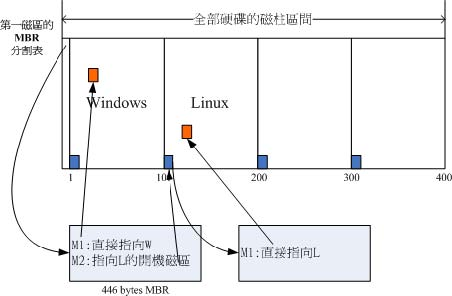
\includegraphics[width=0.55\textwidth]{boot.jpg}
	\caption{开机管理程序的工作执行示意图}
\end{figure}

在上图中我们可以发现,MBR的开机管理程序提供两个选单,选单一(M1)可以直接加载Windows的核心档案来开机; 选单二(M2)则是将开机管理工作交给第二个分区的启动扇区(boot sector)。当使用者在开机的时候选择选单事时,那举整个开机管理工作就会交给第二分区的开机管理程序了。当第二个开机管理程序启动后,该开机管理程序内(上图中)仅有一个开机选单,因此就能够使用Linux的核心档案来开机啰。 这就是多重引导的工作情况啦!我们将上图作个总结:

\begin{itemize}
	\item 每个分区都拥有自己的启动扇区(boot sector)
	\item 图中的系统槽为第一及第二分区,
	\item 实际可开机的核心档案是放置到各分区内的!
	\item loader叧会讣识自己的系统槽内的可开机核心档案,以及其他loader而已;
	\item loader可直接转向或者是间接将管理权转交给另一个管理程序。
\end{itemize}

那现在请你想一想,为什么人家常常说:『如果要安装多重引导, 最好先安装Windows再安装Linux』呢?这是因为:
\begin{itemize}
	\item Linux在安装的时候,你可以选择将开机管理程序安装在MBR或各别分区槽的启动扇区, 而且Linux的loader可以扃劢设定选单(就是上图的M1, M2...),所以你可以在Linux的boot loader里面加入Windows开机的选项;
	\item Windows在安装的时候,他的安装程序会主动的覆盖掉MBR以及自己所在分区的启动扇区,你没有选择的机会,而且他没有让我们自己选择选单的功能。
\end{itemize}

因此,如果先安装Linux再安装Windows的话,那MBR的开机管理程序就叧会有Windows的项目,而且会有Linux的项目 (因为原本在MBR内的Linux的开机管理程序就会被覆盖掉)。 那需要重新安装Linux一次吗?当然不需要,你只要用尽各种方法来处理MBR的内容即可。例如利用全中文的spfdisk(http://spfdisk.sourceforge.net/)软件来安装认识Windows/Linux的管理程序,也能够利用Linux的救援模式(secure mode)来挽救MBR即可。\footnote{详情可参考本节Windows、linux引导修复}

\subsubsection{UEFI+GPT}
由于现在win8、win10系统的用户较多,为了在使用linux的同时也能维持windows系统优秀的用户体验,我们这里讲解在最新的系统启动技术下(支持快速启动)的相关知识,以指导建立分区和安装系统。

UEFI启动是一种新的主板引导项,正被看做是有近20多年历史的BIOS的继任者。顾名思义,快速启动是可以提高开机后操作系统的启动速度。由于开机过程中UEFI的介入,使得Win 8以上的系统的开机进入系统的方式将不同于传统的开机流程。在SSD颠覆了电脑开机慢的问题之后,UEFI+Win10(也可以是其他系统)再一次颠覆我们对于开机速度的概念。

在UEFI+GPT下,计算机启动的过程就简单的多了。大概如下:计算机启动后,BIOS(EFI)将寻找第一个可启动的设备(通常为硬盘),而后从MBR(GPT)中载入启动程序,然后把控制交给这段代码。

\begin{figure}[H]
	%\usepackage{float}
	\centering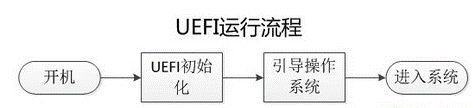
\includegraphics[width=0.8\textwidth]{uefi.png}
	\caption{UEFI运行流程}
\end{figure}

在MBR硬盘中,分区信息直接存储于主引导记录(MBR)中(主引导记录中还存储着系统的引导程序)。但在GPT硬盘中,分区表的位置信息储存在GPT头中。

\textbf{UEFI启动对比BIOS启动的优势}

\begin{enumerate}
	\item 安全性更强
	
	UEFI启动需要一个独立的分区,它将系统启动文件和操作系统本身隔离,可以更好的保护系统的启动。即使系统启动出错需要重新配置,我们只要简单对启动分区重新进行配置即可。而且,对于win8系统,它利用UEFI安全启动以及固件中存储的证书与平台固件之间创建一个信任源,可以确保在加载操作系统之前,近能够执行已签名并获得认证的“已知安全”代码和启动加载程序,可以防止用户在根路径中执行恶意代码。
	
	\item 启动配置更灵活
	
	EFI启动和GRUB启动类似,在启动的时候可以调用EFIShell,在此可以加载指定硬件驱动,选择启动文件。比如默认启动失败,在EFIShell加载U盘上的启动文件继续启动系统。
	
	\item 支持容量更大
	
	传统的BIOS启动由于MBR的限制,默认是无法引导超过2.1TB以上的硬盘的。随着硬盘价格的不断走低,2.1TB以上的硬盘会逐渐普及,因此UEFI启动也是今后主流的启动方式。
\end{enumerate}

\subsection{分区的相关知识}

\subsection{多系统的安装}

\subsubsection{U盘启动盘的制作}

获取一个启动盘是安装的第一步,一般我们为了方便快捷我们选择使用U盘做启动盘。Windows启动盘随处可见,制作简单,我们不再赘述,我们这里简要讲解一下如何使用Universal-USB-Installer制作Ubuntu启动盘。

\textbf{Universal-USB-Installer}是一个非常好用的制作Linux启动盘的工具,体积小,质量高,操作简单。\footnote{下载地址:}

除此之外,我们还要准备正版的Ubuntu镜像,一般我们从官网下载或者从可信任的镜像站下载。\footnote{下载地址:}
\begin{enumerate}

	\item 首先将U盘中有价值的文档备份,因为烧录U盘启动盘的过程可能会将U盘格式化,导致文件丢失。
	
	\item 插入U盘后运行烧录软件Universal-USB-Installer。
	
	\item 点击同意之后点开下拉菜单,选择Ubuntu。
	
	\item 之后点击Browse(浏览),找到存放Ubuntu14.04镜像的地址,确认后选择所要安装的U盘,并调节预留存储变动的空间。\footnote{注意:Set a Persistent file size for storing changes 是选择一个固定的文件存储空间,即如果你登入系统后,对系统有任何更改,将保存到U盘中,如果选择0,则不会保存。有优点也有缺点。具体可见官网给予的解释。http://www.pendrivelinux.com/what-is-persistent-linux/}

	\item 点击create之后,点击是即可进行烧录。
\end{enumerate}

至此,已经完成了Ubuntu系统启动盘的制作,非常容易。

如果你需要制作一张盘上同时可以引导多个操作系统的安装程序,你可以参考如下教程(地址:)

\subsubsection{win8(EFI)与Ubuntu14.04双系统的安装}
刘博

win8在efi引导下ubuntu的安装(b2)
(1)	在EFI(BIOS)中关闭secure boot(安全模式),目的是为了能在机器中安装非windows系统。

(2)在windows下分出30~50G的分区(具体视个人需要和机器的物理内存而定,一般交换空间大小与物理内存大小相同),下面为详细步骤:
右键我的电脑“管理”
点击磁盘管理
选择一个剩余空间较多的分区,如我的D盘,右击,压缩卷,压缩出40~50G的空间,不必新建硬盘分区,即不需要分配硬盘驱动器号。

(3)从Ubuntu官方网站上下载64位Ubuntu14.04的镜像,之后将制作好的优盘启动盘插入电脑,重新启动后更改启动选项,选择从usb HDD(usb硬盘)启动。选择“try but notinstall” 
(4)进入后可能会黑屏,这时候不要紧张,点击键盘上的亮度增加键,一般键盘上会有亮度增加标识,直接按亮度增加键或者按 Fn+亮度增加键,之后屏幕会逐渐亮起来。(这是安装有Nvida显卡的win8系统的通病)
(5)注意此时要选择其他选项: 
(6)再在Ubuntu安装过程中设置文件系统种类及其大小(新分区只能从空闲分区中往外分,如我们刚刚从D盘中分出的30~50G的空间):

<1>先分出200M 给“\\boot”设置为“主分区” ,文件系统为“ext4” 
<2>再分出20G给“\\” 设置为 “逻辑分区”(win8设置成主分区也可,因为UEFI支持超过4个主分区) ,文件系统为“ext4”  
<3>再分 10G (看用户需要)给“\\home”,设置为逻辑分区(win8设置成主分区也可,因为UEFI支持超过4个主分区),此分区在 Ubuntu系统所在分区 损坏时,其中的数据,仍可以保留。
<4>在分出 相当于物理内存大小的空间给“swap”,作为交换空间。
<5>注意要将启动器的位置安装在“\\boot”所在分区 

(7)此时重启后出现引导菜单无法引导进入win8,只能够引导进入Ubuntu,不要着急,此属正常现象,只需在BIOS中打开“secure boot”或者刚刚启动时按Fx键(选择启动项的快捷键),选择从“操作管理员”或者从“windows8”启动,或者从<EFI>/<boot>/<Microsoft>/<windows8.EFI>这条路径启动。进入win8后,用easybcd2.2(一个软件) 修复启动项(一定要提前备份启动项)。
(8)重新启动,在BIOS中关闭“secure boot”,打开快速启动,保存并重新启动。
(9)此时重新启动默认进入win8。刚开机时开机按Fx键(选择启动项的快捷键),选择 从Ubuntu启动,即可进入Ubuntu。
至此,win8 efi引导下ubuntu的安装 结束,双系统安装完毕。

\subsubsection{Q\&A}
\begin{enumerate}
	\item 进入Ubuntu安装界面的时候出现黑屏现象
	
	原因:安装有Nvida显卡的win8的通病
	
	解决方法:点击键盘上面的亮度增加键,即可点亮屏幕
	\item 安装完成系统后,无法进入Ubuntu系统,只能进入windows系统
	
	原因:默认启动时无法自动引导至Ubuntu系统
	
	解决方法:开机时通过更改启动项,更改所启动的系统
	\item 进入Ubuntu系统之后无法挂载windows系统下的硬盘
	
	原因:由于win8、win10有快速启动功能,在关机时,即会将硬盘分区锁定,所以关机后,启动至Ubuntu系统时不能挂载windows的硬盘分区,若windows重新启动,则不会对硬盘分区进行锁定
	
	解决方法:先开机至windows,之后重新启动,选择启动项启动到Ubuntu系统,此时即可访问windows的NTFS格式的硬盘分区,即可实现对硬盘的共用
\end{enumerate}

\subsubsection{WINDOWS引导修复}


1.将制作好的老毛桃u盘启动盘插入电脑中,打开电脑,在看到开机启动画面时按下相应的快捷键进入,在出现的页面中选择u盘启动即可进入到老毛桃u盘启动盘主界面,然后使用上下方向键将光标移动至“【02】运行老毛桃Win2003PE增强版(装机推荐)”按下回车键;如下图所示:

2.当进入到winpe系统后双击pe桌面上的“windows启动引导修复”工具,在弹出的窗口中点击“开始修复”,如下图所示:

3.接着系统就会自动的进行系统引导修复,当修复完成后会建立一个报告;如下图所示:

4.通过修复后的报告我们可以查看到修复后的结果;如下图所示:

接下来只要进行重启系统即可正常进入windows系统桌面了。

\subsubsection{Linux引导修复}

GRUB是一个来自GNU的多操作系统启动程序。GRUB是多启动规范的实现,他允许用户可以在计算机内同时拥有多个操作系统,并在计算机启动时选择希望运行的操作系统。GRUB可用于选择操作系统分区上的不同内核,也可用于向这些内核传递启动参数。在UBUNTU中,默认的存储位置是/BOOT/GRUB,因为我们只是单纯的进行修改与学习,所以我们利用例如GEDIT进行对GRUB.CFG的修改具体命令行参数为进行操作之后可以对GRUB.CFG进行修改。

\begin{enumerate}
	\item 调整默认启动顺序
	在系统启动GRUB进行选择界面时会有这样的界面默认第一个的INDEX为0之后要记住你希望调整的位置之后在GRUB.CFG找到如下代码
	将 SET DEFAULT="0"改为调整位置的INDEX编码
	\item 修复GRUB的步骤
	\subitem 想办法进入到UBUNTU的LIVE CD系统,或者其他较新版本的LIVE CD系统。
	\subitem 打开终端,输入SUDO FDISK -L,查看ID=83的分区,记录下SD[NUM],比如SDA8。
	\subitem 如果上一步中存在多个ID=83的分区,自己想办法确定/分区所在的分区号,并且/BOOT也是和/分区挂载在同一个分区上,比如就是SDA8。
	\subitem 输入SUDO -I,获得ROOT权限。
	\subitem MKDIR /MEDIA/TMP。
	\subitem 将/分区挂载到新建的目录MOUNT /DEV/SDA8 /MEDIA/TMP。
	\subitem 如果以前的系统/BOOT是单独挂载的话,则需要找到/BOOT的分区如SDA7,然后MOUNT /DEV/SDA7 /MEDIA/TMP/BOOT。否则这一步直接跳过去。
	\subitem 接下来准备安装GRUB了,终端输入:GRUB-INSTALL --ROOT-DIRECTORY=/MEDIA/TMP /DEV/SDA。
	\subitem 如果看到INSTALLATION FINISHED, NO ERROR OCCURED之类的信息时表明已经成功了。
	\subitem 此时重启系统,应该可以看到原来的GRUB2引导界面回来了,并且如果有其他系统存在的话,也会显示启动项列表中
\end{enumerate}




\section{Ubuntu的使用}
在Ubuntu上安装开源软件较windows要方便的多,其中最主要的原因就是有了一些安装
\subsection{软件安装之软件源(apt-get)}
 给苹果手机越过狱的同学可能对软件源这个名字不太陌生。软件源是Linux系统的应用程序安装仓库,很多应用软件都会这收录到这个仓库里面。软件源可以是网络服务器,是光盘,甚至是硬盘上的一个目录。
 
 使用软件源安装软件很方便,只需要一条命令.(sudo apt-get install <软件包名> )。
 用软件源安装的软件跟随系统更新,省去很多操作。
 软件源安装的软件都有数字签名,能有效防止恶意软件。
   

  软件源都放在路径为/etc/apt下的sources.list文件内,用文本编辑器打开文件就可以对计算机内的软件源进行添加与删除。
  在终端输入sudo gedit /etc/apt/sources.list,文本编辑器打开的 sources.list就是添加源的文件,只要把找到的源地址添加到文件最后一行,然后在终端运行sudo apt-get update更新配置.
  
   配置文件的格式:
   [软件源地址][发行版地址][包类型]
   
   配置文件类型:
   \begin{itemize}
   	\item main: Canonical公司支持的免费和开源软件
   	\item universe:社区维护的免费和开源软件
   	\item restricted:设备的专有驱动
   	\item multiverse:有版权和合法性问题的软件
   \end{itemize}
   
  我们建议使用中科大或是阿里云的源服务器\footnote{这里放网址,表明版权引用},这两个源更新速度快、软件包全,不过在使用的时候一定要注意对应的Ubuntu版本号,否则会产生一些意想不到的错误。
   
 之前讲过Apt安装软件非常方便,只需要一个命令便可以自动处理依赖关系并安装软件,软件的安装卸载命令如下
 \begin{Code}
 •sudo apt-get install  <软件名> 安装某软件
 •sudo apt-get install  <软件名> --reinstall 重新安装某软件
 •sudo apt-get remove <软件名> 卸载软件
 •sudo apt-get purge <软件名>  卸载某软件,并且清理软件遗留配置文件
 •apt-cache search <字符串> 搜索名称含有字符串的软件
 \end{Code}
 
 apt还有一些其他的命令用来管理软件源和软件包,其中涉及源更新、软件升级、清理软件包等等。
  \begin{Code}
 •sudo apt-get update 更新软件包列表
 •sudo apt-get upgrade 对已安装的软件进行更新
 •sudo apt-get dist-upgrade 对发行版进行升级,可能有新软件包的升级与旧软件包的删除(ubuntu) 发行版升级(debian)
 •sudo do-release-upgrade 手动发行版升级ubuntu
 •sudo apt-get autoremove 移除无用软件包(非手动安装而不被依赖)
 •sudo apt-get autoclean 清理无用的本地安装包缓存
 •sudo apt-get clean 清理所有的本地安装包缓存,缓存路径(/var/cache/apt/archives)
  \end{Code}

 推荐一些图形工具,对于刚接触ubuntu的人可以使用这些工具方便软件的安装和管理。
 
 ubuntu 软件中心:类似于手机的应用商店,一键安装,部分软件付费。
 
 \textbf{新立得软件包管理器}:类似于android的应用商店,可以直接获取软件,一键安装,并且便于软件的更新。
\subsection{软件安装之编译安装}
 当然不是所有的软件都在源上都有,比如在一些开源社区上的工具,往往为了适配更多的平台,都没有直接制作安装包,这时候就要我们自己编译然后再安装到我们的电脑上。这种安装方法虽然有些复杂但也是必要的,
 
\subsubsection{什么是编译安装}
 编译安装简单来说就是根据源码编译出软件(把源码编译成可执行二进制代码),然后对软件进行安装.
 在编译安装之前需要安装编译所需软件包,如gcc,g++,automake,build-essential等.得到的源代码包文件通常为XXX.tar.gz ,XXX.tar.xz,XXX.tar.bz2等格式,实际上是一个压缩文件.
\subsubsection{编译安装流程}
\begin{enumerate}
	\item  tar xvf xxx.tar.gz 解压源码包  
	\item 在终端中进入解压文件目录,并在编译前阅读解压文件中的README和INSTALL文件确定安装方式和所需依赖.
	\item  ./configure  配置编译参数,最常见的是prefix=安装路径,如果不改变则默认把软件安装到系统的文件结构中.
	\item  make 当上一步正确的执行后会生成一个Makefile文件,使用make命令可以对软件源码进行编译
	\item  make install 安装(可能会需要root权限)
\end{enumerate}
 部分软件还会提供make test 这样的测试,在安装前可以运行make test 来测试软件是否编译正确。

\section{shell的使用}
Shell,在计算机科学中又称壳(相对于核来说)。操作系统与外部最主要的接口就叫做shell。
shell管理你与操作系统之间的交互:等待你输入,向操作系统解释你的输入,并且处理各种各样的操作系统的输出结果。shell提供了你与操作系统之间通讯的方式。简单的可以理解成一种可以编译的,可执行的一种语言。
\subsection{常见的shell}
在Linux中,由于命令行的高效率,shell是主要的工作阵地。如今的shell的使用场所已经主要以模拟终端的形式出现在操作系统中,比如windows里的cmd和powershell,Ubuntu里的terminal。上面讲了shell是一种语言,在shell的发展过程中也产生好多个版本,主要有下面这些:
\begin{itemize}
	\item sh :是Steve Bourne在AT\&T贝尔实验室创造的Bourne shell的简称
	\item Bash: 在GUN计划的赞助下免费软件基金会的Brian Fox开发了bash, 是Bourne again shell的简称
	\item Ksh:Ksh shell由AT\&T贝尔实验室的David Korn开发,是sh shell的前身。它是UNIX System V系统中默认和最常用的shell。
	\item Csh: Bill Joy开发了csh shell,并被多数Berkeley UNIX系统(例如Sun Microsystems的产品)作为默认shell。
	\item Tcsh:Tcsh shell是C shell(csh)的开放源代码版本。
	\item Ash:Ash shell是Berkeley UNIX sh shell的简化版本。Kenneth Almquist开发了ash shell。 
	\item Ash shell是可以在系统资源较少的嵌入式系统中使用的一种很好的shell.
	\item Zsh:Zsh 是shell的另一个克隆,提供了很多人性化的设计,非常好用,推荐。
\end{itemize}


shell作为一个脚本语言,主要的元素还是由命令组成,shell命令的使用方法非常简单,从这里我们开始学习shell。

\subsection{Shell命令}

Linux是一个多用户多任务的操作系统,也是一款自由软件,完全兼容POSIX标准,拥有良好的用户界面,支持多种处理器架构,移植方便。Linux 中有大量常用的命令,可以方便我们快速进行操作,值得花时间去掌握。

\subsubsection{命令帮助} 

在linux终端,面对命令不知道怎么用,或不记得命令的拼写及参数时,我们需要求助于系统的帮助文档; linux系统内置的帮助文档很详细,通常能解决我们的问题,我们需要掌握如何正确的去使用它们。
\begin{itemize}
\item 在只记得部分命令关键字的场合,我们可通过man -k来搜索;
\item 需要知道某个命令的简要说明,可以使用whatis;而更详细的介绍,则可用info命令;
\item 查看命令在哪个位置,我们需要使用which;
\item 而对于命令的具体参数及使用方法,我们需要用到强大的man;
\end{itemize}


简要说明命令的作用(显示命令所处的man分类页面):

\begin{Code}
$ whatis command
$ whatis -w "loca*"  //正则匹配:
$ info command       //更加详细的说明文档
\end{Code}

查询命令command的说明文档:

\begin{Code}
$ man command
eg:man date
\end{Code}

在man的帮助手册中,将帮助文档分为了9个类别,对于有的关键字可能存在多个类别中, 我们就需要指定特定的类别来查看;(一般我们查询bash命令,归类在1类中);man页面所属的分类标识(常用的是分类1和分类3)
\begin{enumerate}
\item 用户可以操作的命令或者是可执行文件
\item 系统核心可调用的函数与工具等
\item 一些常用的函数与数据库
\item 设备文件的说明
\item 设置文件或者某些文件的格式
\item 游戏
\item 惯例与协议等。例如Linux标准文件系统、网络协议、ASCⅡ,码等说明内容
\item 系统管理员可用的管理条令
\item 与内核有关的文件
\end{enumerate}


前面说到使用whatis会显示命令所在的具体的文档类别,如下:


\begin{Code}
$ whatis printf
printf               (1)  - format and print data
printf               (1p)  - write formatted output
printf               (3)  - formatted output conversion
printf               (3p)  - print formatted output
printf [builtins]    (1)  - bash built-in commands, see bash(1)
\end{Code}

我们看到printf在分类1和分类3中都有;分类1中的页面是命令操作及可执行文件的帮助;而3是常用函数库说明;如果我们想看的是C语言中printf的用法,可以指定查看分类3的帮助:

\begin{Code}
$ man 3 printf
\end{Code}

\subsubsection{文件、目录管理}  

\textbf{文件创建和删除}

\begin{itemize}
\item 创建:mkdir
\item 删除:rm
\item 删除非空目录:rm -rf file
\item 删除日志 \textbf{rm *log}
\item 移动:mv
\item 复制:cp (复制目录:cp -r )
\end{itemize}

\textbf{目录切换,打印}

\begin{itemize}
	\item 找到文件/目录位置:cd path
	\item 显示当前路径: pwd
	\item 显示当前目录下的文件:ls
	\item 按时间排序,以列表的方式显示目录项:ls -lrt
\end{itemize}

\textbf{查看当前目录下文件个数}

\begin{Code}
    $ find ./ | wc -l
\end{Code}


\textbf{查找文件或目录}
\begin{Code}
    $ find ./ -name '*.o'  //递归查找当前目录及子目录所有的.o文件
\end{Code}

find是实时查找,如果需要更快的查询,可试试locate;locate会为文件系统建立索引数据库,如果有文件更新,需要定期执行更新命令来更新索引库:

\begin{Code}
    $ locate string     //寻找包含有string的路径,
    $ updatedb
\end{Code}    

与find不同,locate并不是实时查找。你需要更新数据库,以获得最新的文件索引信息。

\textbf{查看文件}:cat vi head tail more

\begin{Code}
$ cat -n                // 显示时同时显示行号
$ head -10 filename     // 只看前10行:
$ tail -5 filename      // 显示文件倒数五行
$ diff file1 file2      // 查看两个文件间的差别
\end{Code}

\textbf{文件与目录权限修改}

\begin{itemize}
\item 改变文件的拥有者:chown
\item 改变文件读、写、执行等属性:chmod
\item 递归子目录修改:chown -R user source/
\item 增加脚本可执行权限:chmod +x filename
\end{itemize}


\textbf{创建符号链接/硬链接}

\begin{itemize}
\item ln sourcefile destfile:硬连接;删除一个,将仍能找到;
\item ln -s sourcefile destfile:符号链接(软链接);删除源,另一个无法使用;
\end{itemize}

\subsubsection{进程、作业管理} 

\textbf{ps命令}用于报告当前系统的进程状态。可以搭配kill指令随时中断、删除不必要的程序。ps命令是最基本同时也是非常强大的进程查看命令,使用该命令可以确定有哪些进程正在运行和运行的状态、进程是否结束、进程有没有僵死、哪些进程占用了过多的资源等等,总之大部分信息都是可以通过执行该命令得到的。 

    ps (选项)

选项有很多,常用的如下:
\begin{itemize}
\item a:显示现行终端机下的所有程序,包括其他用户的程序。
\item u:以用户为主的格式来显示程序状况。
\item x:显示所有程序,不以终端机来区分。 
\end{itemize}

\textbf{top命令}可以实时动态地查看系统的整体运行情况,是一个综合了多方信息监测系统性能和运行信息的实用工具。通过top命令所提供的互动式界面,用热键可以管理。

运行 top 命令后,CPU 使用状态会以全屏的方式显示,并且会处在对话的模式,此时用基于 top 的命令,可以控制显示方式。对于进程,平时我们最常想知道的就是哪些进程占用CPU最多,占用内存最多。以下两个命令就可以满足要求:
\begin{itemize}
\item P:根据CPU使用百分比大小进行排序。
\item M:根据驻留内存大小进行排序。
\item i:使top不显示任何闲置或者僵死进程。
\end{itemize}

\textbf{kill命令}用来删除执行中的程序或工作。kill可将指定的信息送至程序。预设的信息为SIGTERM(15),可将指定程序终止。若仍无法终止该程序,可使用SIGKILL(9)信息尝试强制删除程序。程序或工作的编号可利用ps指令或job指令查看。 

一般情况下,我们先用 ps 查找指定进程,然后用 kill 杀掉,如下:

\begin{Code}
ps -ef | grep vim 
root 3268 2884 0 16:21 pts/1 00:00:00 vim install.log 
root 3370 2822 0 16:21 pts/0 00:00:00 grep vim 

kill 3268 
kill 3268
-bash: kill: (3268) - 没有那个进程 
\end{Code}

\textbf{ipcs命令}用于报告Linux中进程间通信设施的状态,显示的信息包括消息列表、共享内存和信号量的信息。 
\begin{itemize}
\item -a:显示全部可显示的信息;
\item -q:显示活动的消息队列信息; 
\item -m:显示活动的共享内存信息; 
\item -s:显示活动的信号量信息。
\end{itemize}

例如:
\begin{Code}
ipcs -a 
------ Shared Memory Segments -------- 
key        shmid   owner perms bytes   nattch status 
0x7401833d 2654208 root  600   4 0 
0x00000000 3145729 root  600   4194304 9      dest 
0x7401833c 2621442 root  600   4       0 
0xd201012b 3080195 root  600   1720    2 
\end{Code}

\textbf{ipcrm命令}用来删除一个或更多的消息队列、信号量集或者共享内存标识。

在linux环境下,任何事物都以文件的形式存在,通过文件不仅仅可以访问常规数据,还可以访问网络连接和硬件。所以如传输控制协议 (TCP) 和用户数据报协议 (UDP) 套接字等,系统在后台都为该应用程序分配了一个文件描述符,无论这个文件的本质如何,该文件描述符为应用程序与基础操作系统之间的交互提供了通用接口。

因为应用程序打开文件的描述符列表提供了大量关于这个应用程序本身的信息,因此通过\textbf{lsof命令}能够查看这个列表对系统监测以及排错将是很有帮助的。 主要有下面这些选项:
\begin{itemize}
\item -a:列出打开文件存在的进程; 
\item -c<进程名>:列出指定进程所打开的文件; 
\item -d<文件号>:列出占用该文件号的进程; 
\item +d<目录>:列出目录下被打开的文件; 
\item -i<条件>:列出符合条件的进程。(4、6、协议、:端口、 @ip ) 
\item -p<进程号>:列出指定进程号所打开的文件;
\end{itemize}
\textbf{jobs命令} 用于显示Linux中的任务列表及任务状态,包括后台运行的任务。该命令可以显示任务号及其对应的进程号。其中,任务号是以普通用户的角度进行的,而进程号则是从系统管理员的角度来看的。一个任务可以对应于一个或者多个进程号。 

其中,输出信息的第一列表示任务编号,第二列表示任务所对应的进程号,第三列表示任务的运行状态,第四列表示启动任务的命令。 

在Linux系统中执行某些操作时候,有时需要将当前任务暂停调至后台,或有时须将后台暂停的任务重启开启并调至前台,这一序列的操作将会使用到 jobs、bg、和 fg 三个命令以及两个快捷键来完成。\textbf{ctrl + z} 可以将一个正在前台执行的命令放到后台,并且暂停。

\begin{Code}
fg %jobnumber  # 将后台中的命令调至前台继续运行
               #(%jobnumber是通过jobs命令查到的后台正在执行的命令的序号(不是pid))
bg %jobnumber  # 将一个在后台暂停的命令,变成继续执行。
\end{Code}

\subsubsection{网络命令} 

\textbf{ifconfig命令}被用于配置和显示Linux内核中网络接口的网络参数。用ifconfig命令配置的网卡信息,在网卡重启后机器重启后,配置就不存在。要想将上述的配置信息永远的存的电脑里,那就要修改网卡的配置文件了。

\textbf{iptables命令}是Linux上常用的防火墙软件,是netfilter项目的一部分。可以直接配置,也可以通过许多前端和图形界面配置。 

\textbf{route命令}用来显示并设置Linux内核中的网络路由表,route命令设置的路由主要是静态路由。直接在命令行下执行route命令来添加路由,不会永久保存,当网卡重启或者机器重启之后,该路由就失效了;可以在/etc/rc.local中添加route命令来保证该路由设置永久有效。

\textbf{netstat命令}用来打印Linux中网络系统的状态信息,可让你得知整个Linux系统的网络情况。可以显示相关的网络信息,如接口/网卡状态(-i),路由表(-r),网络连接(-a),tcp相关选项(-t),udp相关选项(-u),按各个协议统计(-s)。例如:

\begin{Code}
netstat -a #列出所有端口 
netstat -at #列出所有tcp端口 
netstat -au #列出所有udp端口 
netstat -l #只显示监听端口 
netstat -lt #只列出所有监听 tcp 端口 
netstat -lu #只列出所有监听 udp 端口 
netstat -lx #只列出所有监听 UNIX 端口
\end{Code}

\textbf{tcpdump命令}是一款sniffer工具,它可以打印所有经过网络接口的数据包的头信息,也可以使用-w选项将数据包保存到文件中,方便以后分析。如下:

\begin{Code}
tcpdump host 210.27.48.1                # 截获所有210.27.48.1 的主机收到的和发出的所有的数据包
tcpdump tcp port 23 host 210.27.48.1    # 获取主机210.27.48.1接收或发出的telnet包
tcpdump udp port 123                    # 对本机的udp 123 端口进行监视
\end{Code}

\textbf{scp命令}可以将本地localpath指向的文件上传到远程主机的path路径,或者遍历下载path路径下的整个文件系统,到本地的localpath:

\begin{Code}
$ scp localpath ID@host:path
$ scp -r ID@site:path localpath
\end{Code}

\subsubsection{其它命令} 

\textbf{free命令}可以显示当前系统未使用的和已使用的内存数目,还可以显示被内核使用的内存缓冲区。
\begin{itemize}
\item uname -a   \# 查看内核/操作系统/CPU信息
\item hostname   \# 查看计算机名
\item env        \# 查看环境变量
\item uptime     \# 查看系统运行时间、用户数、负载
\end{itemize}

\textbf{useradd命令}用于Linux中创建的新的系统用户。useradd可用来建立用户帐号。帐号建好之后,再用passwd设定帐号的密码,而可用\textbf{userdel}删除帐号。使用useradd指令所建立的帐号,实际上是保存在/etc/passwd文本文件中。

新建一个管理员用户admin,可以用下面命令:

\begin{Code}
useradd -u 0 -o admin
\end{Code}

-u 因为系统用户的用户号为0,故指定用户号为0;因为系统本身存在用户号为0的系统用户,故应该用-o选项,重复使用其他用户的标识号。



\subsubsection{更多阅读} 
[[新建管理员用户](http://www.nowcoder.com/questionTerminal/43d2ccded19445b18ec61069416c299f)]

[为什么计算机的学生要学习 Linux 开源技术](http://www.tinylab.org/why-computer-students-learn-linux-open-source-technologies/) 
   
[工具参考篇](http://linuxtools-rst.readthedocs.org/zh_CN/latest/tool/index.html)  

[Linux 命令大全](http://man.linuxde.net/)  

[学会使用命令帮助](http://linuxtools-rst.readthedocs.io/zh_CN/latest/base/01_use_man.html)  

\subsection{脚本编写}
通常我们把上面这些命令根据一定的语法,组合之后成为一个shell文件,赋予执行权限之后便可以进行自动化操作,这个文件我们称作脚本文件。下面我么通过下面几个方面简单地讲解一下如何编写脚本文件。

建立一个文件并将扩展名修改为.sh,之后用任何文本编辑器打开,键入便开始编写脚本了。

\subsubsection{一个简单的脚本}
这里我们引用《鸟哥的私房菜》的习惯。
鸟哥主要将整个程序的撰写分成数段,大致是这样:

\begin{Code}
	[root@www ~]# mkdir scripts; cd scripts 
	[root@www scripts]# vi sh01.sh 
	#!/bin/bash 
	# Program: 
	# This program shows "Hello World!" in your screen. 
	# History: 
	# 2005/08/23 VBird First release 
	PATH=/bin:/sbin:/usr/bin:/usr/sbin:/usr/
	local/bin:/usr/local/sbin:~/bin export 
	PATH 
	echo -e "Hello World! \a \n" exit 0


1. 第一行 #!/bin/bash 在宣告这个脚本使用的 shell 名称: 因为我们使用的是 bash ,所以,必须要以『 #!/bin/bash 』来宣告这个档案内的语法使用 bash 的语法!那举当这个程序被执行时,他就能够加载 bash 的相关环境配置文件 (一般来说就是 non-login shell 的 ~/.bashrc), 幵且执行 bash 来使我们底下的指令能够执行!这很重要的!(在很多状况中,如果没有设定好这一行, 那举该程序很可能会无法执行,因为系统可能无法判断该程序需要使用什么 shell 来执行啊!)

2. 程序内容的说明: 整个脚本当中,除了第一行的『 #! 』』是用来宣告 shell 的之外,其他的 # 都是『批注』用途! 所以上面的程序当中,第二行以下就是用来说明整个程序的基本数据。一般来说, 建议你一定要养成说明该脚本的:1. 内容不功能; 2. 版本信息; 3. 作者不联络方式; 4. 建档日期;5. 历史纪录 等等。这将有助于未来程序的改写与 debug 呢!

3. 主要环境变量的宣告: 建议务必要将一些重要的环境变量设定好,鸟哥个人认为, PATH 与 LANG (如果有使用到输出相关的信息时) 是当中最重要的! 如此一来,则可让我们这支程序在运行时,可以直接下达一些外部指令,而不必写绝对路径呢!比较好啦!

4. 主要程序部分 就将主要的程序写好即可!在这个例子当中,就是 echo 那一行啦!

5. 执行成果告知 (定义回传值) 
一个指令的执行成功与否,可以使用 \$? 这个发量来观察~ 那么我们也可以利用 exit 这个指令来让程序中断,并且回传一个数值给系统。 在我们这个例子当中,鸟哥使用 exit 0 ,这代表离开脚本幵且回传一个 0 给系统, 所以我执行完这个脚本后,若接着下达 echo \$? 则可得到 0 的值喔! 更聪明的读者应该也知道了,呵呵!利用这个 exit n (n 是数字) 的功能,我们还可以自定义错误讯息, 让这支程序发得更加的 smart 呢!

\end{Code}
接下来透过刚刚上头介绍的执行方法来执行看看结果吧!
\begin{Code}
	[root@www scripts]# sh sh01.sh
	Hello World !
\end{Code}
\subsubsection{好的脚本习惯}
在一些环境的设定上面,毕竟每个人的环境都不相同,为了取得较佳的执行环境, 我都会自行先定义好一些一定会被用到的环境发量,例如 PATH 这个玩意儿! 这样比较好啦~所以说,建议你一定要养成良好的脚本撰写习惯,在每个脚本的文件头处记录好:
\begin{enumerate}
	\item 脚本的功能;
	\item 脚本的版本信息;
	\item 脚本的作者与联系C方式;
	\item 脚本的版权宣告方式;
	\item 脚本的 History (历史纪录);
	\item 脚本内较特殊的指令,使用『绝对路径』的方式来下达;
	\item 脚本运作时需要的环境发量预先宣告与设定。
\end{enumerate}

除了记录这些信息之外,在较为特殊的程序代码部分,个人建议务必要加上批注说明,可以帮助你非常非常多! 此外,程序代码的撰写最好使用巢状方式,在包覆的内部程序代码最好能以 [tab] 按键的空格向后推, 这样你的程序代码会显的非常的漂亮与有条理!在查阅不 debug 上较为轻松愉快喔! 另外,使用撰写脚本的工具最好使用 vim 而不是 vi ,因为 vim 会有额外的语法检验机制,能够在第一阶段撰写时就发现语法方面的问题喔!

\subsubsection{流程控制}

流程控制是任何编程语言中很常用的部分,在bash中也使用if/else,while,until,for等语句来控制流程。
常见的流程控制用法如下:

用if/else控制:
\begin{Code}
if cmda; then
cmd1;
elif cmdb; then
cmd2;
else cmdc; then
cmd3; 
fi
\end{Code}
用while或until控制:
\begin{Code}
while cmd1; do
cmd2;
done
\end{Code}
for条件语句控制:
\begin{Code}
for name in words; do
cmd;
done

for ( (exp1;exp2;exp3));do
cmd;
done
\end{Code}
case条件语句控制:
\begin{Code}
case word in
part1) cmd1;;
part2) cmd2;;
part3) cmd3;;
esac

\end{Code}

举例:for控制语句与数组

\begin{Code}
a=”1 2 3 4 5 a b c”

for I in $a; do
echo $i
done


a=(1 2 3 4 5 a b c)
for ( (i=0;i<10;++i) );do
echo $i
echo ${a[i]}
done
\end{Code}

在这个例子中,有\$符号,\$与其它字符魔术变量,魔术变量对应着特定的语义,如下:

\begin{Code}
$#		argc
$0		argv[0]
$1		argv[1]
${11}	argv[11]
$?		上一句的返回值
$$  		当前bash进程的PID
$-		当前bash的参数
$*		作为一个整体的参数
$@		分词后的参数
\end{Code}


\subsubsection{输入输出}

在 Bash 命令执行的过程中,主要有三种输出入的状况,分别是:

\begin{Code}
	1. 标准输入;代码为 0 ;或称为 stdin ;使用的方式为 <
	2. 标准输出:代码为 1 ;或称为 stdout;使用的方式为 1>
	3. 错误输出:代码为 2 ;或称为 stderr;使用的方式为 2>
\end{Code}

在shell里我们使用”>”和”<”两个符号来重定向输入与输出流,比如:

\begin{Code}	
	ls > file_list		输出到一个文件,覆盖原来的文件
	ls >> file_list       输出重定向到一个文件,追加原来的文件
\end{Code}

重定向符号与标准错误重定向规则如下:

\begin{Code}
	重定向符号:
	>	输出重定向到一个文件或设备 覆盖原来的文件
	>!	输出重定向到一个文件或设备 强制覆盖原来的文件
	>>	输出重定向到一个文件或设备 追加原来的文件
	<	反向输出输入重定向
	标准错误重定向符号:
	2>	将一个标准错误输出重定向到一个文件或设备 覆盖原来的文件
	2>>	将一个标准错误输出重定向到一个文件或设备 追加到原来的文件
	2>&1将一个标准错误输出重定向到标准输出
	>&	将一个标准错误输出重定向到一个文件或设备 覆盖原来的文件
	|&	将一个标准错误 管道 输送 到另一个命令作为输入
\end{Code}
在最后一条规则里面提到了管道这个名词,管道的符号为“|”,其作用是拼接多个程序的输入与输出,即将前一个程序的输出输入到下一个程序作为下一个程序的输入。

假设我们想要知道 /etc/ 底下有多少档案,那么可以利用 ls /etc 来查阅,不过,因为 /etc 底下的档案太多,导致一口气就将屏幕塞满了,从而不知道前面输出的内容是啥。此时,我们可以透过 less 指令的协助,利用:
\begin{Code}
	[root@linux ~]# ls -al /etc | less
\end{Code}
如此一来,使用 ls 指令输出后的内容,就能够被 less 读取, 并且利用 less 的功能,我们就能够前后翻动相关的信息了!

注意:这个管线命令“|” 仅能处理经由前面一个指令传来的正确信息,也就是 standard output( stdout ) 的信息,对于 stdandard error 并没有直接处理的能力,请记得。

创建文件:
\begin{Code}
	touch newfile
	> newfile
	
	echo “something” > file
\end{Code}
\subsubsection{脚本编写实践}
\begin{Code}
#!/bin/bash
#=======================================================
# Agent2D-3.1.0 start script
# RoboCup2D @ Anhui Unversity of Technology
# Bugs or Suggestions please mail to guofeng1208@163.com
#=======================================================


if [ -z "$LD_LIBRARY_PATH" ]
then
LD_LIBRARY_PATH=.
else
LD_LIBRARY_PATH=.:$LD_LIBRARY_PATH
fi

export LD_LIBRARY_PATH


host="localhost"
port=6000
coach_port=6002
teamname="YuShan2015"

player="./YuShan2015_Player"
coach="./YuShan2015_Coach"

config="./data/player.conf"
coach_config="./data/coach.conf"
config_dir="./data/formations-dt"

opt="--player-config ${config} --config_dir ${config_dir}"
coachopt="--coach-config ${coach_config} --use_team_graphic on"


sleeptime=0.5
posnum=0
count=12


usage()
#usage函数
#显示下面的内容直至EOF
{
	cat << EOF
	
	Usage: $0  [options]

	Options:
	-help               Show help infomation
	-h      (IP)        Special server host address
	-p      (port)      Special the server port number of player
	-t      (Name)      Special teamname
	-c      (number)    Special player amount(start with 1)
	-n      (number)    Special player position number(Not uniform)
	EOF
}


if [ $# -eq 1 -a "$1" = "-help" ]
#如果参数数量=1且$1=-help执行usage(-a表示两个条件同时成立)
then
usage
exit 0
fi


while getopts "h:p:t:c:n:" flag
#当输入上的字符是h p t c n中的一个时将其值赋予flag
do
case "$flag" in
h)
host=$OPTARG
;;
p)
port=$OPTARG
coach_port=$((port+2))
;;
t)
teamname=$OPTARG
;;
c)
count=$OPTARG
;;
n)
posnum=$OPTARG
;;
*)
echo "Error cmdline option"
usage
exit 1
esac
done
#当$flag为h时令当前值赋予host


opt="${opt} -h ${host} -p ${port} -t ${teamname}"
coachopt="${coachopt} -h ${host} -p ${coach_port} -t ${teamname}"
#已经定义的参数搭配


# the limit of core dump file size 
ulimit -f unlimited


if [ $posnum -ne 0 ]
#参数$posnum是否不等于0
then
case $posnum in
1)
${player} ${opt} -g -n $posnum &
;;
12)
${coach} ${coachopt}  &
;;
*)
${player} ${opt} -n $posnum  &
;;
esac

exit 0
fi
#当$posnum为1时执行${player} ${opt} -g -n $posnum,即球员的部分
#当$posnum为12时执行${coach} ${coachopt},即教练的部分
#其余的部分执行${player} ${opt} -n $posnum,即球员的部分

i=1

while [ ${i} -le ${count} ]
#${i}小于等于${count}时
do
case ${i} in
1)
echo "team $teamname: Start Player $i"
${player} ${opt} -g &
;;
12)
echo "team $teamname: Start Coach"
${coach} ${coachopt} &
;;
*)
echo "team $teamname: Start Player $i"
${player} ${opt} &
;;
esac

sleep $sleeptime
i=$((i+1))
done
#利用while中的i=$((i+1))使11个球员和一个教练都能参与
#当${i}为1时显示“team $teamname: Start Player $i”执行 ${player} ${opt} -g,即球员的部分
#当${i}为12时时显示"team $teamname: Start Coach"执行 ${coach} ${coachopt},即教练的部分
#当${i}为其它值时输出"team $teamname: Start Player $i"执行 ${player} ${opt}
#$为后台执行
exit 0
\end{Code}

